% !TEX root = thesis.tex
% !TEX encoding = UTF-8 Unicode
\chapter{Analysis}\label{chapterAnalysis}

\begin{equation}
E = mc^2
\label{Einstein}
\end{equation}


% Option p and no other
% => that means: put it on a page with other figures
% Alternatives would be h (here), t (top) and b (bottom) or any
% combination of those like [htbp].
\begin{figure}[p]
\centering
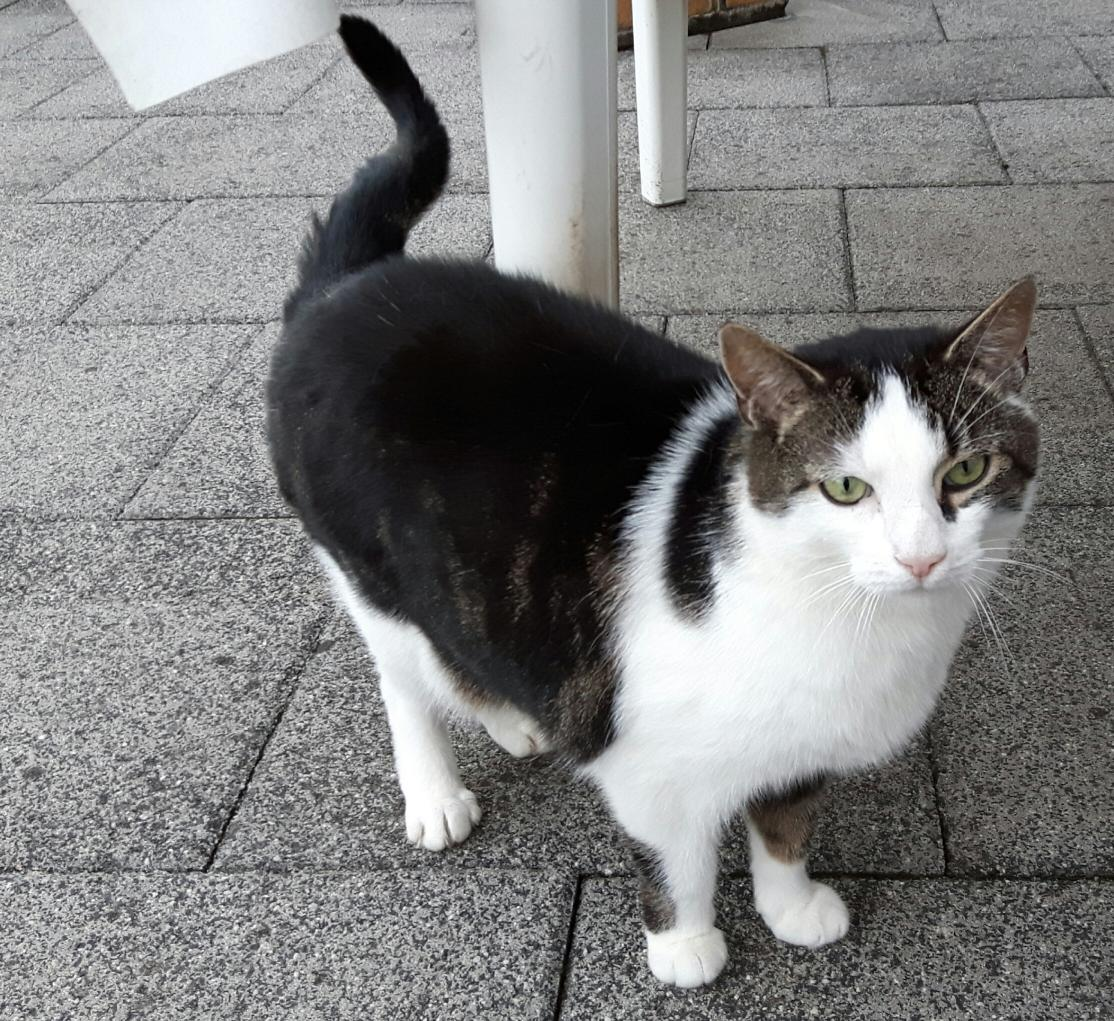
\includegraphics{img/Dala}
\label{img:cat}
\caption{My cat in 2018}
\end{figure}

\blindmathtrue\Blindtext\Blindtext




\begin{figure}[p]
\centering
% Scale the image so it takes up 50% of the width of the text body.
% Height is scaled accordingly.
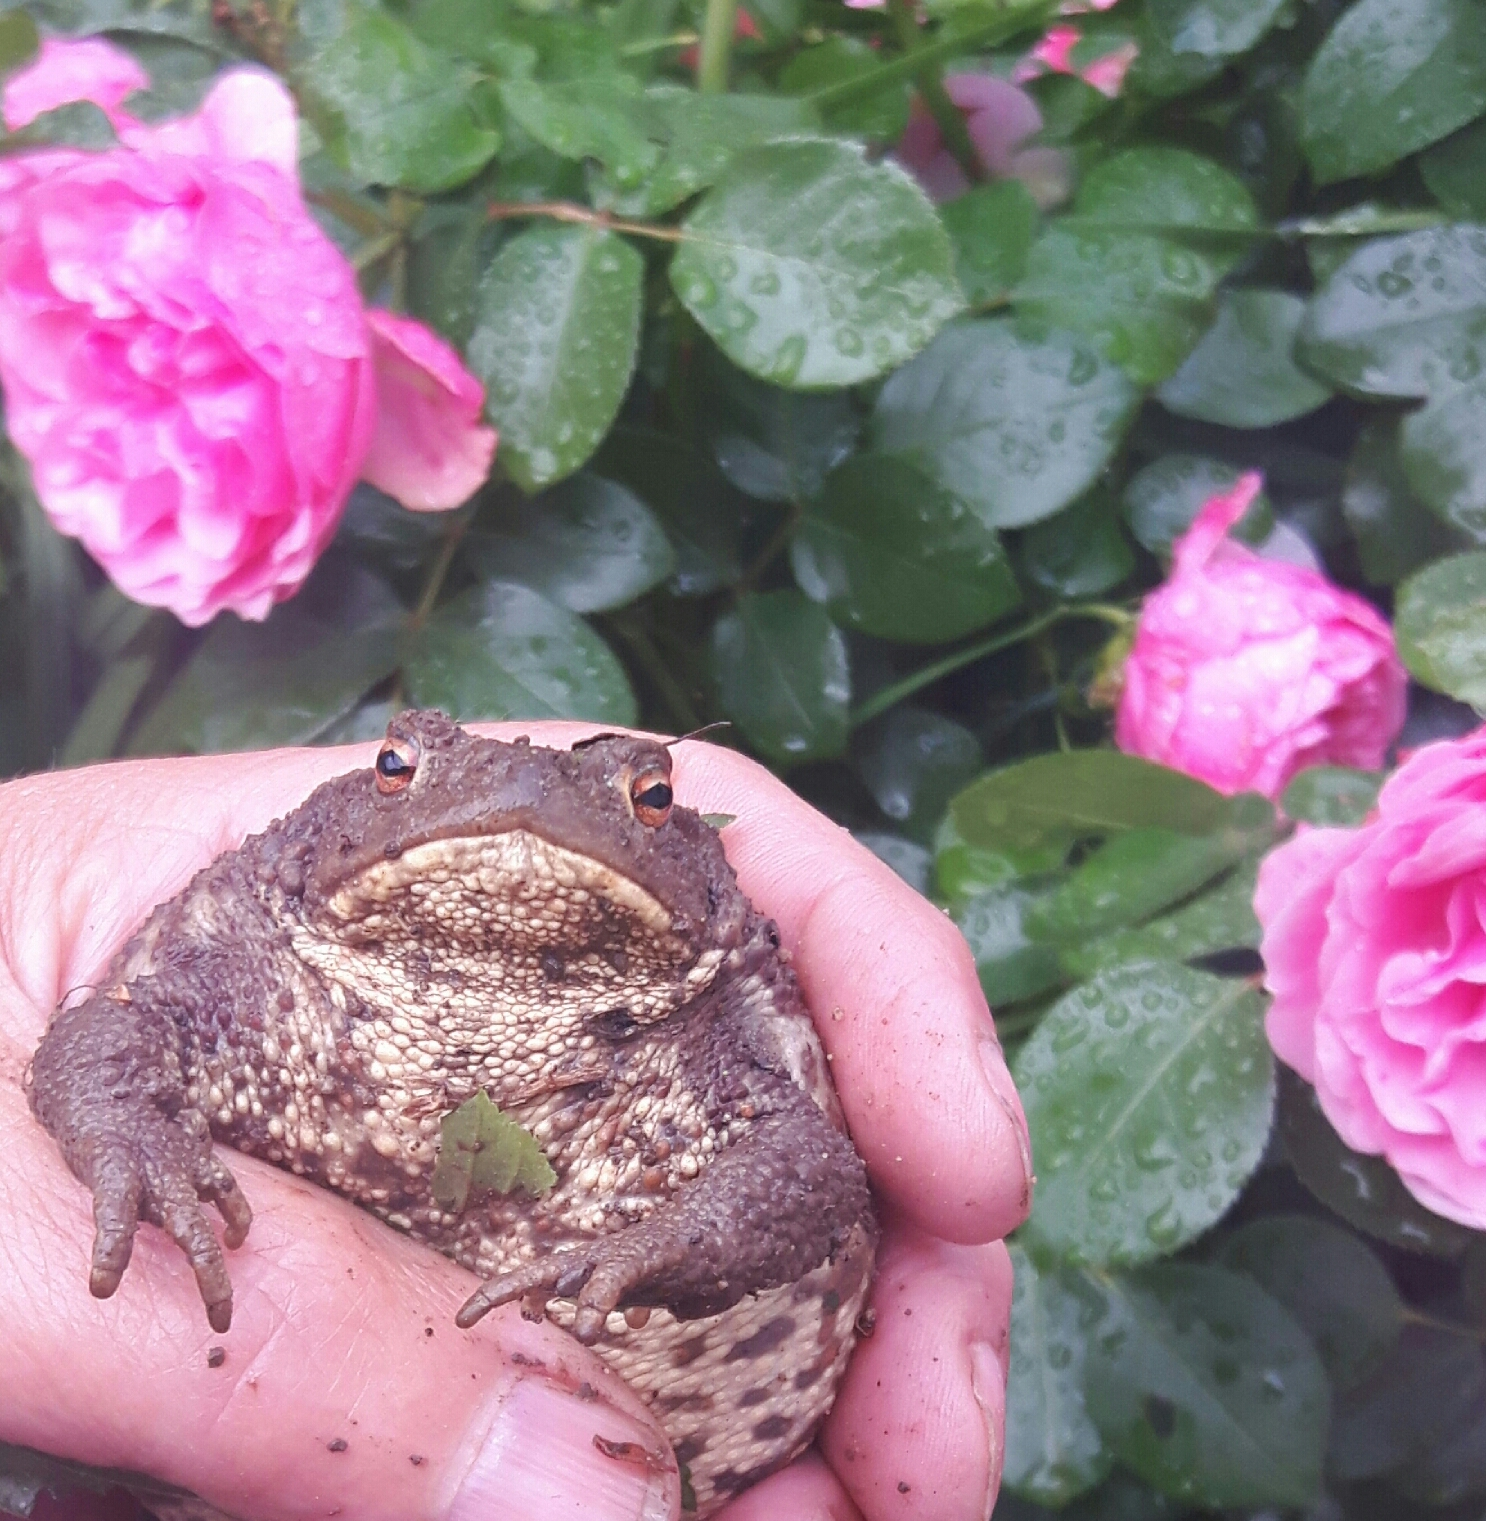
\includegraphics[width=0.5\textwidth]{img/toad}
\label{img:toad}
\caption{A toad found in the garden.}
\end{figure}
